\chapter{Context}
\label{spec:ch:context}

This bachelor thesis is done by Simon Barras and supervised by Frederic Bapst and Jean Hennebert.
The customer Paolo Calafiura is a physicist and computer scientist at the \acrfull{lbl}.
To do this project, I am moving to Berkeley, California, for ten weeks.
The goal is to improve the performance of the project Celeritas, which is a particle physics simulation software accelerated by \acrshort{gpu}s.




\section{Celeritas}
\label{spec:ch:context:celeritas}

The project Celeritas~\cite{Celeritas-Project} is a particle physics simulation software that can be integrated with Geant4~\cite{Geant4} using the Celeritas's library but it can still be used standalone with a limited use for now.
Geant4 is a toolkit for the simulation of the path of particles through matter.
It is used by many simulation software in the field of particle physics.
The fact is that Geant4 is not accelerated by \acrshort{gpu}s and the purpose of Celeritas is to optimize the performance by using them for the propagation and interaction with matter of the resulting photons, electrons and positrons after a collision.



\section{Physics Simulation}
\label{spec:ch:context:physics-simulation}

This project simulates the path of the particles in the detector for any experiment.
Actually, the two main customers are \acrshort{cms} and \acrshort{atlas}, the two made their experiments at the \acrfull{cern} with the \acrfull{lhc}.
The aim is to verify that the measured data are correct but it is also useful to calibrate the detector.
In fact, the simulation is also used to compute the resulting error if there is a lack of precision in a detector.
To find the path of the particles, the software uses the algorithm of Prince Dormand~\cite{princeDormand}, a member of the family Runge-Kutta~\cite{Runge-Kutta-methods}, to solve differential equations.

The \acrfull{atlas} experiment tracks the path of particles in the detector and produces coordinates points where particles traverse the sensors.
Figure \ref{spec:fig:context:physics-simulation:lhc} represents this experiment.
\begin{figure}[ht]
    \centering
    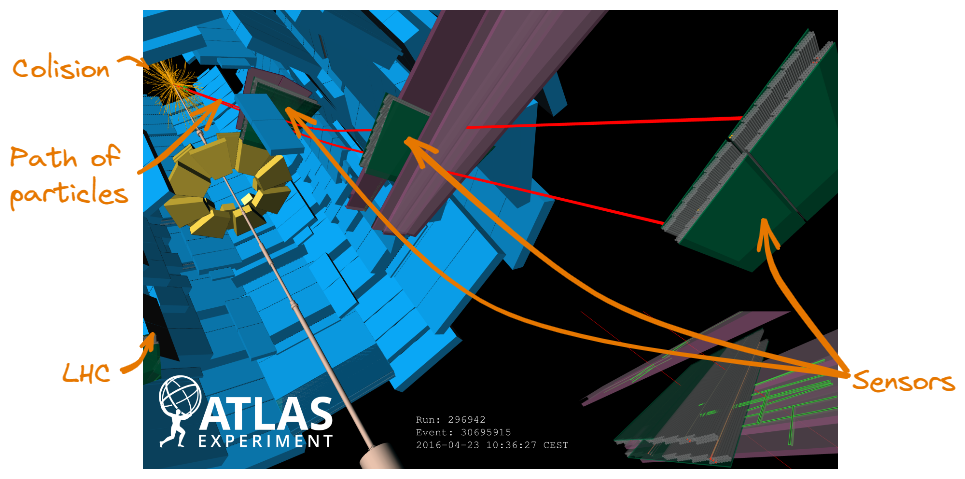
\includegraphics[width=0.9\textwidth]{05-resources/img/spec/experiment-atlas.excalidraw.png}
    \caption{ATLAS experiment at CERN~\cite{atlas-experiment}}
    \label{spec:fig:context:physics-simulation:lhc}
\end{figure}


\section{Lawrence Berkeley National Laboratory}
\label{spec:ch:context:lbl}

The \acrfull{lbl} is a national laboratory in Berkeley, California.
It is managed and operated by the University of California for the \acrfull{doe}.
Since the lab takes part of the \acrshort{doe}, it includes nearly all the research is public and open source.
The lab is situated in the hills of Berkeley and it is composed of many buildings and has a beautiful view of the San Francisco Bay \ref{spec:fig:context:lbl:lab-view}.

\begin{figure}[ht]
    \centering
    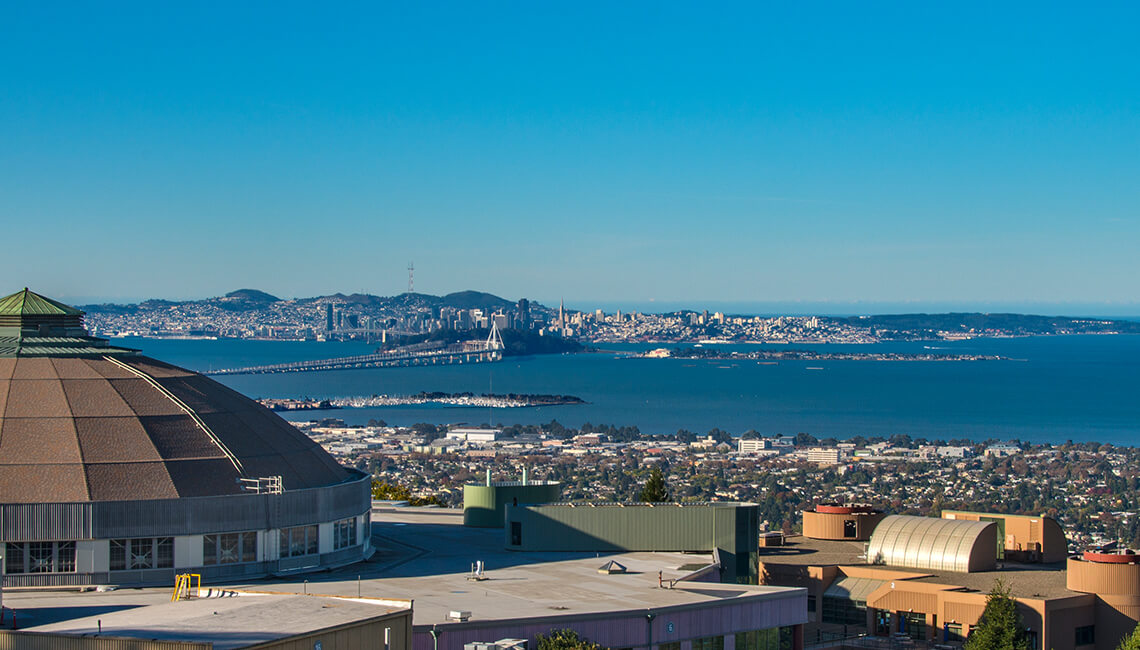
\includegraphics[width=0.8\textwidth]{05-resources/img/spec/lab-view.jpg}
    \caption{Lawrence Berkeley National Laboratory}
    \label{spec:fig:context:lbl:lab-view}
\end{figure}


The Physics and X-Ray Science Group, where the project is done, is situated in building 50f.


\section{The Need}
\label{spec:ch:context:need}

Celeritas already accelerates Geant4 by using \acrshort{gpu}s.
However, the team wants to improve the performance to be able to reduce the time of a simulation.
Before the bachelor thesis, one track is assigned to one \acrshort{gpu}'s thread and there is no collaboration between them.
When the code is profiled with \acrshort{gpu} activated, the distribution of the time is mainly taken by two parts of the code.
The first one is handled by the interaction with the detector geometry to know where in, 3D space, the particle is situated.
During the profiling, it is operated by vecGeom~\cite{VecGeom}.
The second part is the computation of a differential equation using dormant prince~\cite{princeDormand}.
The team wants to improve both but the bachelor thesis will focus on the second one.
